\chapter{Asychroniczny debugger}

W tym rozdziale zamierzam przedstawić zasadę działania wykorzystanego asynchronicznego debuggera na tle narzędzi oferowanych przez JVM. Zamierzam nakreślić problemy oraz sposoby ich rozwiązywania oraz pokazać dlaczego sposób perysytencji komunikatów jest kluczowy dla minimalizacji wpływu debuggera na debugowaną aplikacje. 

%---------------------------------------------------------------------------

\section{Techniki i narzędzia służących do debuggowania}

W tym podrozdziale przedstawię techniki oraz narzędzia służące analizie i debugowaniu aplikacji które udostępnia ekosystem JVM. Zamierzam również pokazać dlaczego narzędzia te są niewystrczające do debugowania programów asychronicznych.

\subsection{Histria działania jako klucz do rozwiązania problemu}

//TODO opisać to szerzej i zmienić tytuł.

\subsection{Historia wywołania a wątki}

//TODO opisac mechanizm analizy stosu wywołań. Pokazać że poza stosem nie mamy innych informacji

\subsection{Wyjątki i ich analiza}
Duża część błędów w programie kończy się rzuceniem wyjątku. Poza informacją o rodzaju wyjątku oraz komunikatem błędu JVM udostępnia nam stack trace.

\begin{quote}
A Stack Trace is a list of method calls from the point when the application was started to the point where the exception was thrown. The most recent method calls are at the top.~\cite{javaProgramming}
\end{quote} 

Stack trace jest niezwykle przydatny przy śledzeniu wywołania gdyż błędy często biorą się ze złego kontekstu wywołania metody (np. wykorzystanie niewłaściwej metody czy nieskończona rekurusja). Dzięki jego analizie jesteśmy w stanie odtworzyć historie wywołań oraz znaleźć kontekst w którym wyjątek został rzucony. Co więcej analiza stack trace'ów pozwala nam na odtworzenie w pewnych sytuacjach parametrów metody czy wartości pól w obiektach.
Niestety stack trace udostępnia nam tylko stos wywołań metod w pojedynczym wątku. Logika (potok logiki) w aplikacjach asychronicznych jest przeważnie rozrzucony po wielu wątkach. Przykładowy stack trace z applikacji w fameworku Akka:

\begin{quote}
TODO wyjątek
\end{quote}

Załączony listing daje nam informacje o stosie wywołań od odebrania ostatniej wiadomości. W przeważającej liczbie przypadków są to informacje niewystarczające gdyż przeważnie nie pozawala nam to na odtworzenie cyklu wiadomości które doprowadziły do powstania wyjątku.

\subsection{Tracing}

Jest to dość proste i naiwne podejście do debugowania polegające logowaniu tekstowych komunikatów zawierających informacje o stanie aplikacji w danym punkcie oraz późniejszej analizie (przeważnie post mortem). Podstawową wadą tego rozwiązania jest konieczność ponownej kompilacji kodu dla każdej fali dodawania kolejnych logów. Często informacje potrzebne do diagnozy problemu nie dają się łatwo zalogować czy to z powodu swojego rozmiary czy struktury. Po poprawieniu błędów programiści często zapominają o usunięciu wszystkich logowanych komunikatów co zaśmieca logi czy kod źródłowy a nawet potrafi być przyczyną problemów.
Rozwiązanie mimo swojej prosty ma szereg zalet. Nie wymaga żadnych specjalistycznych narzędzi ani umiejętności. Posiada także całkiem mały wpływ na wykonanie aplikacji lecz w przypadku aplikacji wielowątkowych wymaga zastosowania bardziej zaawansowanych technik (takich jak dedykowany plik dla każdego wątku).

Umiejętnie stosowany tracing pozwala nam śledzić historię działania aplijakacji. Niestety jest to metoda dość prymitywna i w przypdaku bardziej zaawansowowanych problemów jest niewystarczająca.
 
Mimo swej prostoty rozwiązanie to jest szeroko stosowane przez programistów. W przypadku aplikacji asychronicznych często jest jednym dostępnym sposobem debugowania. 

\subsection{Instrumentacja kodu}

TODO Pisać o tym???
Instrumentacja kodu jest przeważnie wykorzystywana do zautomatyowanego tracingu.

\subsection{Debugger}
Debugger jest programem do dynamicznej analizy wykonania innych programów. 
\begin{quote}
    With the magic of including debugging symbols in the executable, the debugger gives the illusion of executing the program line by line of source code, instead of instruction by instruction of compiled machine code~\cite{artOfDebugging}
\end{quote}
Odwzorowanie kodu maszynowego na kod źródłowy jest skomplikowanym zadaniem, zwłaszcza dla języków wysokopoziomowych. Współczesne debuggery opierają swoje działanie o mechanizm breakpointów czyli definicji miejsc w których wykonanie programu powinno zostać wstrzymane (czasem tylko w celu zalogowania komunikatu - debugger może być także wykorzystany do tracing'u). Po wstrzymaniu działania użytkownik może przeglądać wartości zmiennych, pól czy w bardziej zaawansowanych debuggerach ewaluować wyrażenia.
Debugger pozwala także na sterowanie wykonaniem programu. Poza komendami które nie ingerują w normalne wykonanie programu (Step in, Step out, Step into itp.) pozwala także na np. pownowe wykonanie funkcji (drop frame). Debugger jest doskonałym narzędziem zarówno do naprawiania problemów jak i do zapoznania się z instniejącym kodem.



Niestety debuggery dostępne dla aplikacji działających na JVM posiadają to samo ograniczenie co   analiza wyjątków. Są skuteczne tylko do analizy logiki w ramach pojedynczego wątku. Jest to spowodowane architekturą JVM oraz udostępnianymi przez nią narzędziami.


\section{Java Debug Platform Achitecture}

W tym podroździale zamierzam przedstawić JDPA którę jest podstawowym narzędziem do budowy debuggerów dla aplikacji działących na JVM. Zamierzam również przedstawić narzędzia i właściwości które zamierzam wykorzystać w dalszej części swojej pracy.

\subsection{Architektura}

Jako że każdy debugger jest odzielną aplikacją, Java Platform Debugger Architecture składa się z trzech koponentów przedstawionych na wykresie:

\includegraphics{imgs/jdpa}

\subsubsection{JVM TI: instrumentacja JVM} 

Java™ Virtual Machine Tool Interface służy instrumentacji debuggej JVM.

\begin{quote}
The JVMTM Tool Interface (JVM TI) is a programming interface used by development and monitoring tools. It provides both a way to inspect the state and to control the execution of applications running in the JavaTM virtual machine (VM). \cite{jvmtiSpec}
\end{quote}

Nie jest to tylko narzędzie do debugowania ale może być także podstawą dla tworzenia innych narzedzi takich jak np. profilery.

Aspektem który nas najbardziej interesuje jest niskopoziomowa obsługa breakpointów. Mechanizm działania jest podzielony na 2 etapy:

\begin{enumerate}
\item Deklaracja breakpointu
\item Obsługa eventu wygenerowanego przez breakpoint (tu następuje decyzja czy zatrzymać wykonywanie czy nie)
\end{enumerate}
JVM TI pozwala nam także na dostęp do zmiennych lokalnych oraz parametrów metod. Pozwoli nam to na przechwytywanie przesłanych komunikatów bez udziału debbugera a co za tym idzie przyspieszenie całego procesu, gdyż komunikacja między dwiema aplikacjami jest kosztowna.


\subsubsection{JDWP: protokół transportowy}

Java Debug Wire Protocol: protokół transportowy wykożystywany do komunikacji między maszyną wirtualną (JVM TI) a debuggerem (lub innym programem takim jak profiler). W asychronicznym debuggerze korzystamy z imlementacji dostarczanej przez Java Debug T. W wiekszości przypadków komunikacja jest schowana za warstwą abstrakcji implementują JDI. Więcej informacji możemy znaleść w specyfikacji\cite{jwdpSpec}

\subsubsection{JDI: wysokopoziomowe API}

Wysokopoziomowe API służace do tworzenia debuggerów i innych narzędzi programistycych (np. profilerów). JDI jest interfesjem udostępnianym przez implementacje JDWP i służy do wysokopoziomowej komunikacji z debuggowaną maszyną wirtualną. Podobnie jak JDWP jest zaimplementowany przez JDT i będzie stanowić podstawę dla omawianego asynchronicznego debuggera.
Zawiera metody pozwalające na: \begin{enumerate}
\item deklarowanie breakpointów
\item obsługę eventów (np. zatrzymanie na breakpoint'cie)
\item dostęp do obiektów (parametrów metod, zmiennych lokalnych czy statycnych pól),
\item wywoływanie metod i tworzenie nowych instancji
\item sterowanie wywołaniem aplikacji
\end{enumerate} Większość wymienionych metod zostanie wykorzystana do stworzenia asychronicznego debugera.


% Dalsza część jest mocno pogądowa i nie nadaje się za bardzo do czytania (poza tytułami rozdziałów



\section{Zasada dzialania}

W tym podrozdziale zamierzam przedstawić zasadedziałania asychronicznego debuggera oraz nakreślić  miejsca które będą przedmiotem tej pracy.

\subsection{Asychrnoniczna historia wywołań}
TODO
\subsection{Historia komunikatów}
TODO
\subsection{Budowanie historii komunikatów}

TODO

\subsection{Asychroniczne debuggowanie aplikacji aktorowych: Akka}

\section{debugowanie na JVM}

W tym podrozdziale zamierzam przedstawić JVM w kontekście debugowania aplikacji asynchronicznych. Zmierzam pokazać że potok wywoływania kodu maszynowego różni się koncepcyjnie od potoku przetwarzania komunikatów przez aplikację asynchroniczne. Zamierzam także przestawić właściwości Java Platform Debugger Architecture na których opiera się działania Asychronicznego Debuggera.

\subsection{JVM: wątki}

TODO - opisać stosowość i przypisanie do wątku. Pokazać dlaczego rozdzięk między logiką opartą na komunikatach a na wywołaniach metody

